% Options for packages loaded elsewhere
% Options for packages loaded elsewhere
\PassOptionsToPackage{unicode}{hyperref}
\PassOptionsToPackage{hyphens}{url}
\PassOptionsToPackage{dvipsnames,svgnames,x11names}{xcolor}
%
\documentclass[
  man]{apa7}
\usepackage{xcolor}
\usepackage{amsmath,amssymb}
\setcounter{secnumdepth}{-\maxdimen} % remove section numbering
\usepackage{iftex}
\ifPDFTeX
  \usepackage[T1]{fontenc}
  \usepackage[utf8]{inputenc}
  \usepackage{textcomp} % provide euro and other symbols
\else % if luatex or xetex
  \usepackage{unicode-math} % this also loads fontspec
  \defaultfontfeatures{Scale=MatchLowercase}
  \defaultfontfeatures[\rmfamily]{Ligatures=TeX,Scale=1}
\fi
\usepackage{lmodern}
\ifPDFTeX\else
  % xetex/luatex font selection
\fi
% Use upquote if available, for straight quotes in verbatim environments
\IfFileExists{upquote.sty}{\usepackage{upquote}}{}
\IfFileExists{microtype.sty}{% use microtype if available
  \usepackage[]{microtype}
  \UseMicrotypeSet[protrusion]{basicmath} % disable protrusion for tt fonts
}{}
\makeatletter
\@ifundefined{KOMAClassName}{% if non-KOMA class
  \IfFileExists{parskip.sty}{%
    \usepackage{parskip}
  }{% else
    \setlength{\parindent}{0pt}
    \setlength{\parskip}{6pt plus 2pt minus 1pt}}
}{% if KOMA class
  \KOMAoptions{parskip=half}}
\makeatother
% Make \paragraph and \subparagraph free-standing
\makeatletter
\ifx\paragraph\undefined\else
  \let\oldparagraph\paragraph
  \renewcommand{\paragraph}{
    \@ifstar
      \xxxParagraphStar
      \xxxParagraphNoStar
  }
  \newcommand{\xxxParagraphStar}[1]{\oldparagraph*{#1}\mbox{}}
  \newcommand{\xxxParagraphNoStar}[1]{\oldparagraph{#1}\mbox{}}
\fi
\ifx\subparagraph\undefined\else
  \let\oldsubparagraph\subparagraph
  \renewcommand{\subparagraph}{
    \@ifstar
      \xxxSubParagraphStar
      \xxxSubParagraphNoStar
  }
  \newcommand{\xxxSubParagraphStar}[1]{\oldsubparagraph*{#1}\mbox{}}
  \newcommand{\xxxSubParagraphNoStar}[1]{\oldsubparagraph{#1}\mbox{}}
\fi
\makeatother

\usepackage{color}
\usepackage{fancyvrb}
\newcommand{\VerbBar}{|}
\newcommand{\VERB}{\Verb[commandchars=\\\{\}]}
\DefineVerbatimEnvironment{Highlighting}{Verbatim}{commandchars=\\\{\}}
% Add ',fontsize=\small' for more characters per line
\usepackage{framed}
\definecolor{shadecolor}{RGB}{241,243,245}
\newenvironment{Shaded}{\begin{snugshade}}{\end{snugshade}}
\newcommand{\AlertTok}[1]{\textcolor[rgb]{0.68,0.00,0.00}{#1}}
\newcommand{\AnnotationTok}[1]{\textcolor[rgb]{0.37,0.37,0.37}{#1}}
\newcommand{\AttributeTok}[1]{\textcolor[rgb]{0.40,0.45,0.13}{#1}}
\newcommand{\BaseNTok}[1]{\textcolor[rgb]{0.68,0.00,0.00}{#1}}
\newcommand{\BuiltInTok}[1]{\textcolor[rgb]{0.00,0.23,0.31}{#1}}
\newcommand{\CharTok}[1]{\textcolor[rgb]{0.13,0.47,0.30}{#1}}
\newcommand{\CommentTok}[1]{\textcolor[rgb]{0.37,0.37,0.37}{#1}}
\newcommand{\CommentVarTok}[1]{\textcolor[rgb]{0.37,0.37,0.37}{\textit{#1}}}
\newcommand{\ConstantTok}[1]{\textcolor[rgb]{0.56,0.35,0.01}{#1}}
\newcommand{\ControlFlowTok}[1]{\textcolor[rgb]{0.00,0.23,0.31}{\textbf{#1}}}
\newcommand{\DataTypeTok}[1]{\textcolor[rgb]{0.68,0.00,0.00}{#1}}
\newcommand{\DecValTok}[1]{\textcolor[rgb]{0.68,0.00,0.00}{#1}}
\newcommand{\DocumentationTok}[1]{\textcolor[rgb]{0.37,0.37,0.37}{\textit{#1}}}
\newcommand{\ErrorTok}[1]{\textcolor[rgb]{0.68,0.00,0.00}{#1}}
\newcommand{\ExtensionTok}[1]{\textcolor[rgb]{0.00,0.23,0.31}{#1}}
\newcommand{\FloatTok}[1]{\textcolor[rgb]{0.68,0.00,0.00}{#1}}
\newcommand{\FunctionTok}[1]{\textcolor[rgb]{0.28,0.35,0.67}{#1}}
\newcommand{\ImportTok}[1]{\textcolor[rgb]{0.00,0.46,0.62}{#1}}
\newcommand{\InformationTok}[1]{\textcolor[rgb]{0.37,0.37,0.37}{#1}}
\newcommand{\KeywordTok}[1]{\textcolor[rgb]{0.00,0.23,0.31}{\textbf{#1}}}
\newcommand{\NormalTok}[1]{\textcolor[rgb]{0.00,0.23,0.31}{#1}}
\newcommand{\OperatorTok}[1]{\textcolor[rgb]{0.37,0.37,0.37}{#1}}
\newcommand{\OtherTok}[1]{\textcolor[rgb]{0.00,0.23,0.31}{#1}}
\newcommand{\PreprocessorTok}[1]{\textcolor[rgb]{0.68,0.00,0.00}{#1}}
\newcommand{\RegionMarkerTok}[1]{\textcolor[rgb]{0.00,0.23,0.31}{#1}}
\newcommand{\SpecialCharTok}[1]{\textcolor[rgb]{0.37,0.37,0.37}{#1}}
\newcommand{\SpecialStringTok}[1]{\textcolor[rgb]{0.13,0.47,0.30}{#1}}
\newcommand{\StringTok}[1]{\textcolor[rgb]{0.13,0.47,0.30}{#1}}
\newcommand{\VariableTok}[1]{\textcolor[rgb]{0.07,0.07,0.07}{#1}}
\newcommand{\VerbatimStringTok}[1]{\textcolor[rgb]{0.13,0.47,0.30}{#1}}
\newcommand{\WarningTok}[1]{\textcolor[rgb]{0.37,0.37,0.37}{\textit{#1}}}

\usepackage{longtable,booktabs,array}
\usepackage{calc} % for calculating minipage widths
% Correct order of tables after \paragraph or \subparagraph
\usepackage{etoolbox}
\makeatletter
\patchcmd\longtable{\par}{\if@noskipsec\mbox{}\fi\par}{}{}
\makeatother
% Allow footnotes in longtable head/foot
\IfFileExists{footnotehyper.sty}{\usepackage{footnotehyper}}{\usepackage{footnote}}
\makesavenoteenv{longtable}
\usepackage{graphicx}
\makeatletter
\newsavebox\pandoc@box
\newcommand*\pandocbounded[1]{% scales image to fit in text height/width
  \sbox\pandoc@box{#1}%
  \Gscale@div\@tempa{\textheight}{\dimexpr\ht\pandoc@box+\dp\pandoc@box\relax}%
  \Gscale@div\@tempb{\linewidth}{\wd\pandoc@box}%
  \ifdim\@tempb\p@<\@tempa\p@\let\@tempa\@tempb\fi% select the smaller of both
  \ifdim\@tempa\p@<\p@\scalebox{\@tempa}{\usebox\pandoc@box}%
  \else\usebox{\pandoc@box}%
  \fi%
}
% Set default figure placement to htbp
\def\fps@figure{htbp}
\makeatother





\setlength{\emergencystretch}{3em} % prevent overfull lines

\providecommand{\tightlist}{%
  \setlength{\itemsep}{0pt}\setlength{\parskip}{0pt}}



 
\usepackage[]{biblatex}
\addbibresource{references.bib}


\usepackage{booktabs}
\usepackage{caption}
\usepackage{longtable}
\usepackage{colortbl}
\usepackage{array}
\usepackage{anyfontsize}
\usepackage{multirow}
\makeatletter
\@ifpackageloaded{caption}{}{\usepackage{caption}}
\AtBeginDocument{%
\ifdefined\contentsname
  \renewcommand*\contentsname{Table of contents}
\else
  \newcommand\contentsname{Table of contents}
\fi
\ifdefined\listfigurename
  \renewcommand*\listfigurename{List of Figures}
\else
  \newcommand\listfigurename{List of Figures}
\fi
\ifdefined\listtablename
  \renewcommand*\listtablename{List of Tables}
\else
  \newcommand\listtablename{List of Tables}
\fi
\ifdefined\figurename
  \renewcommand*\figurename{Figure}
\else
  \newcommand\figurename{Figure}
\fi
\ifdefined\tablename
  \renewcommand*\tablename{Table}
\else
  \newcommand\tablename{Table}
\fi
}
\@ifpackageloaded{float}{}{\usepackage{float}}
\floatstyle{ruled}
\@ifundefined{c@chapter}{\newfloat{codelisting}{h}{lop}}{\newfloat{codelisting}{h}{lop}[chapter]}
\floatname{codelisting}{Listing}
\newcommand*\listoflistings{\listof{codelisting}{List of Listings}}
\makeatother
\makeatletter
\makeatother
\makeatletter
\@ifpackageloaded{caption}{}{\usepackage{caption}}
\@ifpackageloaded{subcaption}{}{\usepackage{subcaption}}
\makeatother
\usepackage{bookmark}
\IfFileExists{xurl.sty}{\usepackage{xurl}}{} % add URL line breaks if available
\urlstyle{same}
\hypersetup{
  pdftitle={Estimating Personal Values in Text},
  pdfauthor={Andrew Demetriou},
  colorlinks=true,
  linkcolor={blue},
  filecolor={Maroon},
  citecolor={Blue},
  urlcolor={Blue},
  pdfcreator={LaTeX via pandoc}}


\title{Estimating Personal Values in Text}
\author{Andrew Demetriou}
\date{}
\begin{document}
\maketitle


\subsection{Pilot Methods}\label{pilot-methods}

\begin{Shaded}
\begin{Highlighting}[]
\CommentTok{\# details for all studies}
\NormalTok{pilot\_2\_demog\_df }\OtherTok{\textless{}{-}}\NormalTok{ pilot\_2\_demog\_dfs }\SpecialCharTok{|\textgreater{}} \FunctionTok{bind\_rows}\NormalTok{(}\AttributeTok{.id =} \StringTok{"study"}\NormalTok{)}

\CommentTok{\# mean age:}
\NormalTok{pilot\_2\_demog\_df }\SpecialCharTok{|\textgreater{}}
  \FunctionTok{summarize}\NormalTok{(}
    \AttributeTok{N =} \FunctionTok{n}\NormalTok{(), }
    \AttributeTok{mean\_age =} \FunctionTok{mean}\NormalTok{(Age), }
    \AttributeTok{sd\_age =} \FunctionTok{sd}\NormalTok{(Age), }
    \AttributeTok{percent\_female =} \FunctionTok{round}\NormalTok{(}\FunctionTok{mean}\NormalTok{(Sex }\SpecialCharTok{==} \StringTok{"Female"}\NormalTok{, }\AttributeTok{na.rm =} \ConstantTok{TRUE}\NormalTok{) }\SpecialCharTok{*} \DecValTok{100}\NormalTok{, }\DecValTok{2}\NormalTok{))}
\end{Highlighting}
\end{Shaded}

\begin{verbatim}
    N mean_age   sd_age percent_female
1 296 36.05068 11.81011          48.65
\end{verbatim}

The average age of participants was 36.1 years (SD = 11.8).\\
The proportion of female participants was 48.6\%.

\subsection{Pilot Results}\label{pilot-results}

\subsubsection{Estimating the number of
raters}\label{estimating-the-number-of-raters}

\begin{Shaded}
\begin{Highlighting}[]
\NormalTok{p1 }\OtherTok{\textless{}{-}} \FunctionTok{plot\_raters}\NormalTok{(}
\NormalTok{  pilot\_2\_lyrics\_by\_row\_dfs[[}\DecValTok{1}\NormalTok{]] }\SpecialCharTok{\%\textgreater{}\%} \FunctionTok{filter}\NormalTok{(n }\SpecialCharTok{\textless{}=} \DecValTok{25}\NormalTok{), }
  \AttributeTok{metric =}\NormalTok{ r, }\StringTok{"Pearson\textquotesingle{}s r"}\NormalTok{, }\AttributeTok{option =} \StringTok{"plasma"}\NormalTok{) }\SpecialCharTok{+} 
  \FunctionTok{geom\_vline}\NormalTok{(}\AttributeTok{xintercept =} \FloatTok{0.9}\NormalTok{, }\AttributeTok{color =} \StringTok{"red"}\NormalTok{, }\AttributeTok{size =}\NormalTok{ .}\DecValTok{4}\NormalTok{, }\AttributeTok{linetype =} \StringTok{"dashed"}\NormalTok{) }

\NormalTok{p2 }\OtherTok{\textless{}{-}} \FunctionTok{plot\_raters}\NormalTok{(}
\NormalTok{  pilot\_2\_lyrics\_by\_row\_dfs[[}\DecValTok{1}\NormalTok{]] }\SpecialCharTok{\%\textgreater{}\%} \FunctionTok{filter}\NormalTok{(n }\SpecialCharTok{\textless{}=} \DecValTok{25}\NormalTok{), }
  \AttributeTok{metric =}\NormalTok{ ICC2k, }\StringTok{"ICC(2,k)"}\NormalTok{, }\AttributeTok{option =} \StringTok{"plasma"}\NormalTok{) }\SpecialCharTok{+}
  \FunctionTok{geom\_vline}\NormalTok{(}\AttributeTok{xintercept =} \FloatTok{0.75}\NormalTok{, }\AttributeTok{color =} \StringTok{"red"}\NormalTok{, }\AttributeTok{size =}\NormalTok{ .}\DecValTok{4}\NormalTok{, }\AttributeTok{linetype =} \StringTok{"dashed"}\NormalTok{) }

\NormalTok{(p1 }\SpecialCharTok{/}\NormalTok{p2) }\SpecialCharTok{+}
    \FunctionTok{plot\_annotation}\NormalTok{(}
    \AttributeTok{title =} \StringTok{"**Figure 2**"}\NormalTok{,}
    \AttributeTok{subtitle =} \StringTok{"*Reliability by Rater n: Lyrics Pilot*"}\NormalTok{, }
    \AttributeTok{caption =} \StringTok{"*Note.* Probability Density for Pearson\textquotesingle{}s r and ICC(2,k)."}\NormalTok{, }
    \AttributeTok{tag\_levels =} \StringTok{\textquotesingle{}A\textquotesingle{}}\NormalTok{) }\SpecialCharTok{+}
  
  \FunctionTok{plot\_layout}\NormalTok{(}\AttributeTok{guides =} \StringTok{"collect"}\NormalTok{) }\SpecialCharTok{\&}
  
  \FunctionTok{theme}\NormalTok{(}\AttributeTok{legend.position =} \StringTok{"right"}\NormalTok{,}
        \AttributeTok{plot.title =} \FunctionTok{element\_markdown}\NormalTok{(}\AttributeTok{hjust =} \DecValTok{0}\NormalTok{), }
        \AttributeTok{plot.subtitle =} \FunctionTok{element\_markdown}\NormalTok{(}\AttributeTok{hjust =} \DecValTok{0}\NormalTok{), }
        \AttributeTok{plot.caption =} \FunctionTok{element\_markdown}\NormalTok{(}\AttributeTok{hjust =} \DecValTok{0}\NormalTok{))}
\end{Highlighting}
\end{Shaded}

\pandocbounded{
\includegraphics[keepaspectratio]{manuscript_files/figure-pdf/unnamed-chunk-17-1.pdf}}

\pandocbounded{\includegraphics[keepaspectratio]{manuscript_files/figure-pdf/unnamed-chunk-18-1.pdf}}

\pandocbounded{\includegraphics[keepaspectratio]{manuscript_files/figure-pdf/unnamed-chunk-19-1.pdf}}

\subsubsection{Exploring annotator sample
strata}\label{exploring-annotator-sample-strata}

\begin{Shaded}
\begin{Highlighting}[]
\NormalTok{p1\_1 }\OtherTok{\textless{}{-}}\NormalTok{ pilot\_2\_lyrics\_agreement\_plots[[}\DecValTok{2}\NormalTok{]]}
\NormalTok{p1\_2 }\OtherTok{\textless{}{-}}\NormalTok{ pilot\_2\_lyrics\_agreement\_plots[[}\DecValTok{3}\NormalTok{]]}
\NormalTok{p1\_3 }\OtherTok{\textless{}{-}}\NormalTok{ pilot\_2\_lyrics\_agreement\_plots[[}\DecValTok{4}\NormalTok{]]}
\NormalTok{p1\_4 }\OtherTok{\textless{}{-}}\NormalTok{ pilot\_2\_lyrics\_agreement\_plots[[}\DecValTok{5}\NormalTok{]]}


\NormalTok{(p1\_1 }\SpecialCharTok{|}\NormalTok{ p1\_2) }\SpecialCharTok{/}\NormalTok{ (p1\_3 }\SpecialCharTok{|}\NormalTok{ p1\_4) }\SpecialCharTok{+}
  
  \FunctionTok{plot\_annotation}\NormalTok{(}
    \AttributeTok{title =} \StringTok{"**Figure 6**"}\NormalTok{,}
    \AttributeTok{subtitle =} \StringTok{"*ICC(2,k) by Schwartz value, by Ethnicity: Lyrics Pilot*"}\NormalTok{, }
    \AttributeTok{caption =} 
         \StringTok{"*Note.* Error bars are 95\% confidence intervals. }
\StringTok{         \textquotesingle{}Self\textquotesingle{} indicates reliability for the value \textquotesingle{}self direction\textquotesingle{}."}\NormalTok{) }\SpecialCharTok{\&}
  
  \FunctionTok{theme}\NormalTok{(}\AttributeTok{plot.title =} \FunctionTok{element\_markdown}\NormalTok{(}\AttributeTok{hjust =} \DecValTok{0}\NormalTok{), }
        \AttributeTok{plot.subtitle =} \FunctionTok{element\_markdown}\NormalTok{(}\AttributeTok{hjust =} \DecValTok{0}\NormalTok{), }
        \AttributeTok{plot.caption =} \FunctionTok{element\_markdown}\NormalTok{(}\AttributeTok{hjust =} \DecValTok{0}\NormalTok{))}
\end{Highlighting}
\end{Shaded}

\pandocbounded{
\includegraphics[keepaspectratio]{manuscript_files/figure-pdf/unnamed-chunk-21-1.pdf}}

\begin{Shaded}
\begin{Highlighting}[]
\NormalTok{p2 }\OtherTok{\textless{}{-}}\NormalTok{ pilot\_2\_speeches1\_agreement\_plots[[}\DecValTok{1}\NormalTok{]]}\SpecialCharTok{+}\FunctionTok{ggtitle}\NormalTok{(}\StringTok{""}\NormalTok{)}
\NormalTok{p3 }\OtherTok{\textless{}{-}}\NormalTok{ pilot\_2\_speeches2\_agreement\_plots[[}\DecValTok{1}\NormalTok{]]}\SpecialCharTok{+}\FunctionTok{ggtitle}\NormalTok{(}\StringTok{""}\NormalTok{)}

\NormalTok{(p2}\SpecialCharTok{/}\NormalTok{p3) }\SpecialCharTok{+} 
  \FunctionTok{plot\_annotation}\NormalTok{(}
    \AttributeTok{title =} \StringTok{"**Figure 7**"}\NormalTok{,}
    \AttributeTok{subtitle =} \StringTok{"*ICC(2,k) by Schwartz value, by Ethnicity: Speeches Pilots 1 and 2*"}\NormalTok{, }
    \AttributeTok{caption =} 
    \StringTok{"*Note.* Error bars are 95\% confidence intervals. }
\StringTok{         \textquotesingle{}Self\textquotesingle{} indicates reliability for the value \textquotesingle{}self direction\textquotesingle{}."}\NormalTok{, }
    \AttributeTok{tag\_levels =} \StringTok{\textquotesingle{}1\textquotesingle{}}\NormalTok{) }\SpecialCharTok{\&}
  
  \FunctionTok{theme}\NormalTok{(}\AttributeTok{plot.title =} \FunctionTok{element\_markdown}\NormalTok{(}\AttributeTok{hjust =} \DecValTok{0}\NormalTok{), }
        \AttributeTok{plot.subtitle =} \FunctionTok{element\_markdown}\NormalTok{(}\AttributeTok{hjust =} \DecValTok{0}\NormalTok{), }
        \AttributeTok{plot.caption =} \FunctionTok{element\_markdown}\NormalTok{(}\AttributeTok{hjust =} \DecValTok{0}\NormalTok{))}
\end{Highlighting}
\end{Shaded}

\pandocbounded{\includegraphics[keepaspectratio]{manuscript_files/figure-pdf/unnamed-chunk-22-1.pdf}}

\begin{Shaded}
\begin{Highlighting}[]
\NormalTok{p1\_1 }\OtherTok{\textless{}{-}}\NormalTok{ pilot\_2\_speeches1\_agreement\_plots[[}\DecValTok{2}\NormalTok{]]}
\NormalTok{p1\_2 }\OtherTok{\textless{}{-}}\NormalTok{ pilot\_2\_speeches1\_agreement\_plots[[}\DecValTok{3}\NormalTok{]]}
\NormalTok{p1\_3 }\OtherTok{\textless{}{-}}\NormalTok{ pilot\_2\_speeches1\_agreement\_plots[[}\DecValTok{4}\NormalTok{]]}
\NormalTok{p1\_4 }\OtherTok{\textless{}{-}}\NormalTok{ pilot\_2\_speeches1\_agreement\_plots[[}\DecValTok{5}\NormalTok{]]}

\NormalTok{(p1\_1 }\SpecialCharTok{|}\NormalTok{ p1\_2) }\SpecialCharTok{/}\NormalTok{ (p1\_3 }\SpecialCharTok{|}\NormalTok{ p1\_4) }\SpecialCharTok{+}
  
  \FunctionTok{plot\_annotation}\NormalTok{(}
    \AttributeTok{title =} \StringTok{"**Figure 8**"}\NormalTok{,}
    \AttributeTok{subtitle =} \StringTok{"*ICC(2,k) by Schwartz value, by Ethnicity: Speeches 1 Pilot*"}\NormalTok{, }
    \AttributeTok{caption =} 
         \StringTok{"*Note.* Error bars are 95\% confidence intervals. }
\StringTok{         \textquotesingle{}Self\textquotesingle{} indicates reliability for the value \textquotesingle{}self direction\textquotesingle{}."}\NormalTok{) }\SpecialCharTok{\&}
  
  \FunctionTok{theme}\NormalTok{(}\AttributeTok{plot.title =} \FunctionTok{element\_markdown}\NormalTok{(}\AttributeTok{hjust =} \DecValTok{0}\NormalTok{), }
        \AttributeTok{plot.subtitle =} \FunctionTok{element\_markdown}\NormalTok{(}\AttributeTok{hjust =} \DecValTok{0}\NormalTok{), }
        \AttributeTok{plot.caption =} \FunctionTok{element\_markdown}\NormalTok{(}\AttributeTok{hjust =} \DecValTok{0}\NormalTok{))}
\end{Highlighting}
\end{Shaded}

\pandocbounded{\includegraphics[keepaspectratio]{manuscript_files/figure-pdf/unnamed-chunk-23-1.pdf}}

\begin{Shaded}
\begin{Highlighting}[]
\NormalTok{p1\_1 }\OtherTok{\textless{}{-}}\NormalTok{ pilot\_2\_speeches2\_agreement\_plots[[}\DecValTok{2}\NormalTok{]]}
\NormalTok{p1\_2 }\OtherTok{\textless{}{-}}\NormalTok{ pilot\_2\_speeches2\_agreement\_plots[[}\DecValTok{3}\NormalTok{]]}
\NormalTok{p1\_3 }\OtherTok{\textless{}{-}}\NormalTok{ pilot\_2\_speeches2\_agreement\_plots[[}\DecValTok{4}\NormalTok{]]}
\NormalTok{p1\_4 }\OtherTok{\textless{}{-}}\NormalTok{ patchwork}\SpecialCharTok{::}\FunctionTok{plot\_spacer}\NormalTok{()}

\NormalTok{((p1\_1 }\SpecialCharTok{/}\NormalTok{ p1\_2) }\SpecialCharTok{|}\NormalTok{ (p1\_3 }\SpecialCharTok{/}\NormalTok{ p1\_4)) }\SpecialCharTok{+}
  \FunctionTok{plot\_annotation}\NormalTok{(}
    \AttributeTok{title =} \StringTok{"**Figure 9**"}\NormalTok{,}
    \AttributeTok{subtitle =} \StringTok{"*ICC(2,k) by Schwartz value, by Political Leaning: Speeches 2 Pilot*"}\NormalTok{, }
    \AttributeTok{caption =} 
         \StringTok{"*Note.* Error bars are 95\% confidence intervals. }
\StringTok{         \textquotesingle{}Self\textquotesingle{} indicates reliability for the value \textquotesingle{}self direction\textquotesingle{}."}\NormalTok{) }\SpecialCharTok{\&}
  
  \FunctionTok{theme}\NormalTok{(}\AttributeTok{plot.title =} \FunctionTok{element\_markdown}\NormalTok{(}\AttributeTok{hjust =} \DecValTok{0}\NormalTok{), }
        \AttributeTok{plot.subtitle =} \FunctionTok{element\_markdown}\NormalTok{(}\AttributeTok{hjust =} \DecValTok{0}\NormalTok{), }
        \AttributeTok{plot.caption =} \FunctionTok{element\_markdown}\NormalTok{(}\AttributeTok{hjust =} \DecValTok{0}\NormalTok{))}
\end{Highlighting}
\end{Shaded}

\pandocbounded{
\includegraphics[keepaspectratio]{manuscript_files/figure-pdf/unnamed-chunk-24-1.pdf}}

\subsubsection{Exploring Quiz Results}\label{exploring-quiz-results}

\begin{Shaded}
\begin{Highlighting}[]
\NormalTok{summarize\_study }\OtherTok{\textless{}{-}} \ControlFlowTok{function}\NormalTok{(df) \{}
\NormalTok{  df }\SpecialCharTok{\%\textgreater{}\%}
    \FunctionTok{summarise}\NormalTok{(}
      \AttributeTok{Q1 =} \FunctionTok{sprintf}\NormalTok{(}\StringTok{"\%d (\%.1f\%\%)"}\NormalTok{, }\FunctionTok{sum}\NormalTok{(Quiz1, }\AttributeTok{na.rm =} \ConstantTok{TRUE}\NormalTok{),}
                      \FunctionTok{mean}\NormalTok{(Quiz1, }\AttributeTok{na.rm =} \ConstantTok{TRUE}\NormalTok{) }\SpecialCharTok{*} \DecValTok{100}\NormalTok{),}
      \AttributeTok{Q2 =} \FunctionTok{sprintf}\NormalTok{(}\StringTok{"\%d (\%.1f\%\%)"}\NormalTok{, }\FunctionTok{sum}\NormalTok{(Quiz2, }\AttributeTok{na.rm =} \ConstantTok{TRUE}\NormalTok{),}
                      \FunctionTok{mean}\NormalTok{(Quiz2, }\AttributeTok{na.rm =} \ConstantTok{TRUE}\NormalTok{) }\SpecialCharTok{*} \DecValTok{100}\NormalTok{),}
      \AttributeTok{Q3 =} \FunctionTok{sprintf}\NormalTok{(}\StringTok{"\%d (\%.1f\%\%)"}\NormalTok{, }\FunctionTok{sum}\NormalTok{(Quiz3, }\AttributeTok{na.rm =} \ConstantTok{TRUE}\NormalTok{),}
                      \FunctionTok{mean}\NormalTok{(Quiz3, }\AttributeTok{na.rm =} \ConstantTok{TRUE}\NormalTok{) }\SpecialCharTok{*} \DecValTok{100}\NormalTok{)}
\NormalTok{    ) }\SpecialCharTok{\%\textgreater{}\%}
    
    \FunctionTok{pivot\_longer}\NormalTok{(}\FunctionTok{everything}\NormalTok{(), }\AttributeTok{names\_to =} \StringTok{"Question"}\NormalTok{, }\AttributeTok{values\_to =} \StringTok{"N\_percent"}\NormalTok{)}
\NormalTok{\}}

\FunctionTok{lapply}\NormalTok{(quiz\_dfs, summarize\_study) }\SpecialCharTok{\%\textgreater{}\%}
  
  \FunctionTok{bind\_rows}\NormalTok{(}\AttributeTok{.id =} \StringTok{"Study"}\NormalTok{) }\SpecialCharTok{\%\textgreater{}\%}
  
  \FunctionTok{pivot\_wider}\NormalTok{(}\AttributeTok{names\_from =}\NormalTok{ Study, }\AttributeTok{values\_from =}\NormalTok{ N\_percent) }\SpecialCharTok{\%\textgreater{}\%}
  
  \FunctionTok{gt}\NormalTok{() }\SpecialCharTok{\%\textgreater{}\%}
  
  \FunctionTok{tab\_header}\NormalTok{(}
    \AttributeTok{title =} \FunctionTok{md}\NormalTok{(}\StringTok{"**Table 4**"}\NormalTok{),}
    \AttributeTok{subtitle =} \FunctionTok{md}\NormalTok{(}\StringTok{"*Pilot Studies: Quiz Item Correctness*"}\NormalTok{)}
\NormalTok{  ) }\SpecialCharTok{\%\textgreater{}\%}
  \FunctionTok{cols\_label}\NormalTok{(}
    \AttributeTok{Question =} \StringTok{"Item"}\NormalTok{,}
    \AttributeTok{lyrics =} \StringTok{"Pilot: Lyrics"}\NormalTok{,}
    \AttributeTok{speeches1 =} \StringTok{"Pilot: Speeches 1"}\NormalTok{,}
    \AttributeTok{speeches2 =} \StringTok{"Pilot: Speeches 2"}
\NormalTok{  ) }\SpecialCharTok{\%\textgreater{}\%}
  \FunctionTok{cols\_align}\NormalTok{(}
    \AttributeTok{align =} \StringTok{"center"}\NormalTok{,}
    \AttributeTok{columns =} \FunctionTok{everything}\NormalTok{()}
\NormalTok{  ) }\SpecialCharTok{\%\textgreater{}\%}
  \FunctionTok{cols\_width}\NormalTok{(}\FunctionTok{everything}\NormalTok{() }\SpecialCharTok{\textasciitilde{}} \FunctionTok{px}\NormalTok{(}\DecValTok{100}\NormalTok{)) }\SpecialCharTok{|\textgreater{}}
  \FunctionTok{tab\_options}\NormalTok{(}
    \AttributeTok{table.font.size =} \DecValTok{12}\NormalTok{,}
    \AttributeTok{heading.align =} \StringTok{"left"}\NormalTok{,}
    \AttributeTok{table.border.top.width =} \FunctionTok{px}\NormalTok{(}\DecValTok{0}\NormalTok{),       }\CommentTok{\# remove top rule}
    \AttributeTok{table.border.bottom.width =} \FunctionTok{px}\NormalTok{(}\DecValTok{0}\NormalTok{),    }\CommentTok{\# remove bottom rule}
    \AttributeTok{table\_body.hlines.width =} \FunctionTok{px}\NormalTok{(}\DecValTok{0}\NormalTok{),   }\CommentTok{\# removes horizontal lines inside body}
    \AttributeTok{table\_body.vlines.width =} \FunctionTok{px}\NormalTok{(}\DecValTok{0}\NormalTok{)    }\CommentTok{\# removes vertical lines}
\NormalTok{  ) }\SpecialCharTok{\%\textgreater{}\%}
  \FunctionTok{tab\_source\_note}\NormalTok{(}
    
    \FunctionTok{md}\NormalTok{(}\StringTok{"*Note.* Entries are number and percentage of participants who answered correctly. Quiz responses were not used to exclude participants in pilot studies."}\NormalTok{))}
\end{Highlighting}
\end{Shaded}

\begin{table}
\caption*{
{\large \textbf{Table 4}} \\ 
{\small \emph{Pilot Studies: Quiz Item Correctness}}
} 
\fontsize{9.0pt}{10.8pt}\selectfont
\begin{tabular*}{\linewidth}{@{\extracolsep{\fill}}>{\centering\arraybackslash}p{\dimexpr 75.00pt -2\tabcolsep-1.5\arrayrulewidth}>{\centering\arraybackslash}p{\dimexpr 75.00pt -2\tabcolsep-1.5\arrayrulewidth}>{\centering\arraybackslash}p{\dimexpr 75.00pt -2\tabcolsep-1.5\arrayrulewidth}>{\centering\arraybackslash}p{\dimexpr 75.00pt -2\tabcolsep-1.5\arrayrulewidth}}
\toprule
Item & Pilot: Lyrics & Pilot: Speeches 1 & Pilot: Speeches 2 \\ 
\midrule\addlinespace[2.5pt]
Q1 & 77 (77.8\%) & 81 (81.8\%) & 78 (79.6\%) \\ 
Q2 & 48 (48.5\%) & 43 (43.4\%) & 42 (42.9\%) \\ 
Q3 & 69 (69.7\%) & 65 (65.7\%) & 69 (70.4\%) \\ 
\bottomrule
\end{tabular*}
\begin{minipage}{\linewidth}
\emph{Note.} Entries are number and percentage of participants who answered correctly. Quiz responses were not used to exclude participants in pilot studies.\\
\end{minipage}
\end{table}

\pandocbounded{
\includegraphics[keepaspectratio]{manuscript_files/figure-pdf/unnamed-chunk-27-1.pdf}}

\printbibliography

\section{References}\label{references}

\printbibliography[heading=none]

\section{Appendix A: Stimuli}\label{appendix-a-stimuli}

\subsection{Lyrics Stimuli}\label{lyrics-stimuli}

Songs were sampled across four ``fuzzy'' strata: (1) Year of release,
based on Musixmatch metadata; (2) Popularity, defined as the frequency
with which an artist appeared on playlists in the Million Playlist
Dataset (MPD); (3) Genre, estimated by topic modeling user-generated
artist tags, which were originally drawn from Last.fm and merged into
the MPD; and (4) Lyric topic, derived from topic modeling a bag-of-words
representation of the lyrics. After selecting the final sample of 2,200
songs, Musixmatch provided the first 30\% of the lyrics for each track
via their API.

The code \textcite{demetriou2024towards} used to sample lyrics can be
found here:
https://anonymous.4open.science/r/lyrics-value-estimators-CE33/1\_stimulus\_sampling/stratified\_sampling.py.

Note: neither the raw lyric data nor the unanonymized repository can be
made available due to limitations in licensing.

\subsubsection{Release Date}\label{release-date}

Release date was determined via Musixmatch metadata, some of which may
contain errors. Metadata included a wide range of release years,
beginning in 1890 (which appeared to include traditional songs
e.g.~Little Drummer Boy). There were a total of 14 bins in 10 equally
spaced year intervals (1890, 1900) \textasciitilde{} (2020, 2030).
Number and percentage of songs that were kept after the manual screening
procedure, by the meta-data year range per year bin are shown in Figure
1 and Table 1.

{\textbf{Figure s-1}\\
\emph{Manual screening outcome by year bin range}}

\begin{Shaded}
\begin{Highlighting}[]
\FunctionTok{make\_removed\_counts}\NormalTok{(lyrics\_df, year\_bin\_range)}
\end{Highlighting}
\end{Shaded}

\pandocbounded{
\includegraphics[keepaspectratio]{manuscript_files/figure-pdf/unnamed-chunk-42-1.pdf}}

{Note. ``remove'' indicates songs excluded due to manual screening
criteria. Bins presented in reverse order of number of songs labelled
``keep''. Each row indicates a decade-range year bin, with x axis labels
showing the observed metadata range per year bin.}

\begin{Shaded}
\begin{Highlighting}[]
\FunctionTok{make\_apa\_freq\_table}\NormalTok{(}
\NormalTok{  lyrics\_df}\SpecialCharTok{|\textgreater{}}\FunctionTok{rename}\NormalTok{(}\StringTok{\textasciigrave{}}\AttributeTok{Year Range}\StringTok{\textasciigrave{}}\OtherTok{=}\NormalTok{ year\_bin\_range),}
  \StringTok{\textasciigrave{}}\AttributeTok{Year Range}\StringTok{\textasciigrave{}}\NormalTok{,}
  \AttributeTok{title =} \FunctionTok{md}\NormalTok{(}\StringTok{"**Table s{-}1**"}\NormalTok{),}
  \AttributeTok{subtitle =} \FunctionTok{md}\NormalTok{(}\StringTok{"*Frequencies by release year bin*"}\NormalTok{)}
\NormalTok{)}
\end{Highlighting}
\end{Shaded}

\begin{table}
\caption*{
{\large \textbf{Table s-1}} \\ 
{\small \emph{Frequencies by release year bin}}
} 
\fontsize{9.0pt}{10.8pt}\selectfont
\begin{tabular*}{\linewidth}{@{\extracolsep{\fill}}lrrr}
\toprule
{Year Range} & Removed & Kept & Total n \\ 
\midrule\addlinespace[2.5pt]
2010–2019 & 222 (43.6\%) & 287 (56.4\%) & 509 \\ 
2000–2009 & 142 (42.3\%) & 194 (57.7\%) & 336 \\ 
1990–1999 & 71 (35.5\%) & 129 (64.5\%) & 200 \\ 
2020–2021 & 47 (27.3\%) & 125 (72.7\%) & 172 \\ 
1980–1989 & 27 (18.1\%) & 122 (81.9\%) & 149 \\ 
1961–1969 & 24 (17.8\%) & 111 (82.2\%) & 135 \\ 
1952–1959 & 23 (17.8\%) & 106 (82.2\%) & 129 \\ 
1970–1979 & 17 (12.2\%) & 122 (87.8\%) & 139 \\ 
1942–1946 & 3 (23.1\%) & 10 (76.9\%) & 13 \\ 
1900–1900 & 1 (20.0\%) & 4 (80.0\%) & 5 \\ 
1925–1929 & 1 (33.3\%) & 2 (66.7\%) & 3 \\ 
1930–1936 & 1 (16.7\%) & 5 (83.3\%) & 6 \\ 
1899–1899 & 0 (0.0\%) & 3 (100.0\%) & 3 \\ 
\bottomrule
\end{tabular*}
\end{table}

{Note. ``Removed'' indicates songs excluded due to manual screening
criteria. Bins presented in reverse order of number of songs removed.
Each row indicates a decade-range year bin, with column Year Range
showing the observed metadata range per year bin.}

\subsubsection{Popularity}\label{popularity}

Popularity was extremely exponentially distributed, with an extreme left
skew. We manually binned to make the quantiles per each of the 7 bins as
similar as possible. Thus, the first bin contained the lowest 40\% of
the population in terms of popularity, while the 7th bin contained the
highest 9\%:

\begin{itemize}
\tightlist
\item
  \textbf{Bin 0:} 1--2 playlist appearances (≤ 40\%)
\item
  \textbf{Bin 2:} 2--3 appearances (41--53\%)
\item
  \textbf{Bin 3:} 3--4 appearances (54--60\%)
\item
  \textbf{Bin 4:} 4--6 appearances (61--70\%)
\item
  \textbf{Bin 5:} 7--14 appearances (71--80\%)
\item
  \textbf{Bin 6:} 15--60 appearances (81--91\%)
\item
  \textbf{Bin 7:} 61--203,345 appearances (top 9\% of artists;
  91--100\%)
\end{itemize}

{\textbf{Figure s-2}\\
\emph{Manual screening outcome by popularity bin percentile range}}

\begin{Shaded}
\begin{Highlighting}[]
\FunctionTok{make\_removed\_counts}\NormalTok{(lyrics\_df, artist\_playlist\_frequency\_bin\_label)}
\end{Highlighting}
\end{Shaded}

\pandocbounded{
\includegraphics[keepaspectratio]{manuscript_files/figure-pdf/unnamed-chunk-44-1.pdf}}

{Note. ``remove'' indicates songs excluded due to manual screening
criteria. Bins presented in reverse order of number of songs labelled
``keep''.}

\begin{Shaded}
\begin{Highlighting}[]
\FunctionTok{make\_apa\_freq\_table}\NormalTok{(}
\NormalTok{  lyrics\_df}\SpecialCharTok{|\textgreater{}}\FunctionTok{rename}\NormalTok{(}\StringTok{\textasciigrave{}}\AttributeTok{Artist Popularity}\StringTok{\textasciigrave{}}\OtherTok{=}\NormalTok{artist\_playlist\_frequency\_bin\_label),}
  \StringTok{\textasciigrave{}}\AttributeTok{Artist Popularity}\StringTok{\textasciigrave{}}\NormalTok{,}
  \AttributeTok{title =} \FunctionTok{md}\NormalTok{(}\StringTok{"**Table s{-}2**"}\NormalTok{),}
  \AttributeTok{subtitle =} \FunctionTok{md}\NormalTok{(}\StringTok{"*Frequencies by artist playlist frequency*"}\NormalTok{)}
\NormalTok{)}
\end{Highlighting}
\end{Shaded}

\begin{table}
\caption*{
{\large \textbf{Table s-2}} \\ 
{\small \emph{Frequencies by artist playlist frequency}}
} 
\fontsize{9.0pt}{10.8pt}\selectfont
\begin{tabular*}{\linewidth}{@{\extracolsep{\fill}}lrrr}
\toprule
{Artist Popularity} & Removed & Kept & Total n \\ 
\midrule\addlinespace[2.5pt]
91\%-100\% & 145 (38.2\%) & 235 (61.8\%) & 380 \\ 
81\%-91\% & 115 (41.2\%) & 164 (58.8\%) & 279 \\ 
<= 40 \% & 80 (31.5\%) & 174 (68.5\%) & 254 \\ 
71\%-80\% & 76 (31.9\%) & 162 (68.1\%) & 238 \\ 
41\%-53\% & 58 (26.7\%) & 159 (73.3\%) & 217 \\ 
61\%-70\% & 53 (23.7\%) & 171 (76.3\%) & 224 \\ 
54\%-60\% & 52 (25.1\%) & 155 (74.9\%) & 207 \\ 
\bottomrule
\end{tabular*}
\end{table}

{Note. ``Removed'' indicates songs excluded due to manual screening
criteria. Bins presented in reverse order of number of songs removed.
Each row indicates a popularity percentile range bin, with column Artist
Popularity showing the observed percentile range per popularity bin.}

\subsubsection{Genre}\label{genre}

\textcite{demetriou2024towards} used topic modelling applied to a
bag-of-words representation of artist-tag data to estimate one of \(25\)
estimated genres for each included artist, which were then applied to
songs. To get the initial pool, \textcite{demetriou2024towards} first
uniformly sampled 60k artists from the Spotify Million Playlist Dataset
(MPD)\autocite{chen2018recsys}, which contains metadata on
\textasciitilde2 million tracks by \textasciitilde300k artists. They
then retrieved the full discographies of these artists via the Spotify
API and cross-checked availability in Musixmatch, yielding a pool of
\textasciitilde510k songs from \textasciitilde15.4k' artists. We used
Latent Dirichlet allocation to create a topic model of the artist tags
in order to derive estimated genres, shown in the ``Top LDA terms of
initial pool'' column of Table 3a.

From this pool, 2,200 songs were selected, and manually screened. As
there is no definitive label for each estimated genre, we derived a
second set of labels aimed at describing the 1,425 artists in the sample
pool, as opposed to the initial 15.4k artist pool. Specifically, we
gathered each unique artist in the 2,200 song sample, and drew the genre
label tags for those artists from using the Spotify and Last.fm APIs. We
then pooled all the artist genre tags for each artist, and estimated the
tf-idf for each tag per genre bin. The top tf-idf terms are shown in the
``Top tf-df terms of sample'' column of table 3a.

\begin{Shaded}
\begin{Highlighting}[]
\FunctionTok{make\_genre\_comparison\_table}\NormalTok{(lyrics\_df,}
  \AttributeTok{title =} \FunctionTok{md}\NormalTok{(}\StringTok{"**Table s{-}4**"}\NormalTok{),}
  \AttributeTok{subtitle =} \FunctionTok{md}\NormalTok{(}\StringTok{"*Comparison of terms of topic tags of initial pool of 15.4k artists, to secondary pool of 2200 songs*"}\NormalTok{)}
\NormalTok{)  }\SpecialCharTok{\%\textgreater{}\%}
  \FunctionTok{cols\_width}\NormalTok{(lda\_genre\_terms }\SpecialCharTok{\textasciitilde{}} \FunctionTok{px}\NormalTok{(}\DecValTok{350}\NormalTok{), artist\_topic\_bin\_labels }\SpecialCharTok{\textasciitilde{}} \FunctionTok{px}\NormalTok{(}\DecValTok{300}\NormalTok{))}
\end{Highlighting}
\end{Shaded}

\begin{table}
\caption*{
{\large \textbf{Table s-4}} \\ 
{\small \emph{Comparison of terms of topic tags of initial pool of 15.4k artists, to secondary pool of 2200 songs}}
} 
\fontsize{9.0pt}{10.8pt}\selectfont
\begin{tabular*}{\linewidth}{@{\extracolsep{\fill}}>{\centering\arraybackslash}p{\dimexpr 262.50pt -2\tabcolsep-1.5\arrayrulewidth}>{\raggedright\arraybackslash}p{\dimexpr 225.00pt -2\tabcolsep-1.5\arrayrulewidth}}
\toprule
Top LDA terms of initial pool & Top tf-ifd terms of sample \\ 
\midrule\addlinespace[2.5pt]
All, dubstep, synthpop, 80s, new wave, post-punk, russian, electropop, Disco, electronic & synthpop / new wave / post-punk / dubstep \\ 
blues, american, USA, Canadian, shoegaze, dream pop, black metal, United States, canada, twee & blues / blues rock / classic blues / black metal \\ 
christian, gospel, worship, arabic, christian rock, spain, cumbia, mexico, mexican, portuguese & christian / worship / gospel / ccm \\ 
country, Soundtrack, Alt-country, americana, danish, turkish, video game music, texas, christmas, Disney & classic country / country / honky tonk / traditional country \\ 
dance, House, trance, electronic, Progressive House, progressive trance, club, electronica, techno, eurodance & eurodance / dance / trance / electronic \\ 
electronic, ambient, experimental, techno, electronica, electro, House, deep house, minimal, downtempo & electronic / ebm / industrial / electronica \\ 
folk, singer-songwriter, acoustic, folk rock, bluegrass, indie folk, norwegian, Norway, argentina, americana & folk / singer-songwriter / folk rock / acoustic \\ 
hardcore, metalcore, metal, hardcore punk, post-hardcore, deathcore, Nu Metal, seen live, melodic hardcore, grindcore & hardcore punk / hardcore / punk rock / deathcore \\ 
heavy metal, metal, celtic, thrash metal, dutch, seen live, irish, Power metal, finnish, bass & metal / power metal / heavy metal / speed metal \\ 
Hip-Hop, rap, hip hop, spotify, underground hip-hop, trap, beats, hiphop, underground rap, instrumental hip-hop & hip hop / rap / underground hip-hop / trap \\ 
instrumental, Classical, piano, Drum and bass, contemporary classical, psytrance, composer, dnb, Drum n Bass, baroque & classical / drum and bass / choral / piano \\ 
japanese, ska, new age, j-pop, J-rock, japan, Asian, anime, chiptune, soca & j-pop / ska / j-rock / rocksteady \\ 
jazz, chillout, lounge, trip-hop, downtempo, swing, Fusion, easy listening, Smooth Jazz, acid jazz & big band / jazz / vocal jazz / swing \\ 
latin, male vocalists, spanish, 90s, italian, salsa, mexico, 00s, 10s, Italy & italian / latin / italian singer-songwriter / latino \\ 
oldies, death metal, comedy, african, Melodic Death Metal, Brutal Death Metal, doo wop, 50s, spoken word, afrobeat & comedy / afrobeats / african / doo-wop \\ 
pop, female vocalists, french, female vocalist, pop rock, france, female, Eurovision, chanson francaise, indonesian & pop / female vocalists / chanson / eurovision \\ 
punk, punk rock, emo, pop punk, post-hardcore, seen live, rock, polish, screamo, chicago & punk rock / pop punk / hardcore punk / ska punk \\ 
reggae, brazilian, dub, dancehall, brasil, brazil, Stoner Rock, mpb, Sludge, Southern Rock & reggae / roots reggae / dancehall / ragga \\ 
rnb, german, rockabilly, power pop, Rock and Roll, germany, rock n roll, deutsch, urban, Deutschrap & rock n roll / rockabilly / r\&b / new jack swing \\ 
rock, psychedelic, hard rock, alternative rock, Progressive rock, Psychedelic Rock, classic rock, Korean, alternative, k-pop & rock / psychedelic rock / k-pop / progressive rock \\ 
seen live, indie, alternative, indie rock, indie pop, rock, british, post-rock, Lo-Fi, australian & indie rock / indie / indie pop / alternative \\ 
soul, funk, r\&b, rhythm and blues, Disco, Greek, rnb, funky, Neo-Soul, northern soul & soul / funk / r\&b / motown \\ 
swedish, guitar, blues rock, lesser known yet streamable artists, United Kingdom, Sweden, england, Flamenco, Jam, Awesome & swedish / swedish pop / blues rock / nordic \\ 
under 2000 listeners, musical, Reggaeton, Colombia, Broadway, hungarian, Musical theatre, musicals, showtunes, trollerier & musicals / broadway / showtunes / shady \\ 
world, Garage Rock, 60s, World Music, garage, traditional, Surf, Need to Rate, Indian, darkwave & sufi / gothic rock / darkwave / indian \\ 
\bottomrule
\end{tabular*}
\end{table}

\textcite{demetriou2024towards} excluded songs if they contained more
than \textgreater= \textasciitilde20\% non-English words, consisted only
of onomatopoeia or nonsense, repeated a single word or phrase, or had
too few words. This process yielded 380 songs. We extended screening
with the same criteria, resulting in 1,200 songs. We used 800 in the
main study and 14 for a pilot. Songs were primarily removed for
containing too many non-English words, or having too few or single
repeated words. Distribution of included songs by genre bin, as well as
results from manual screening procedure are shown in Figure 3.

{\textbf{Figure s-3}\\
\emph{Manual screening outcome by genre}}

\pandocbounded{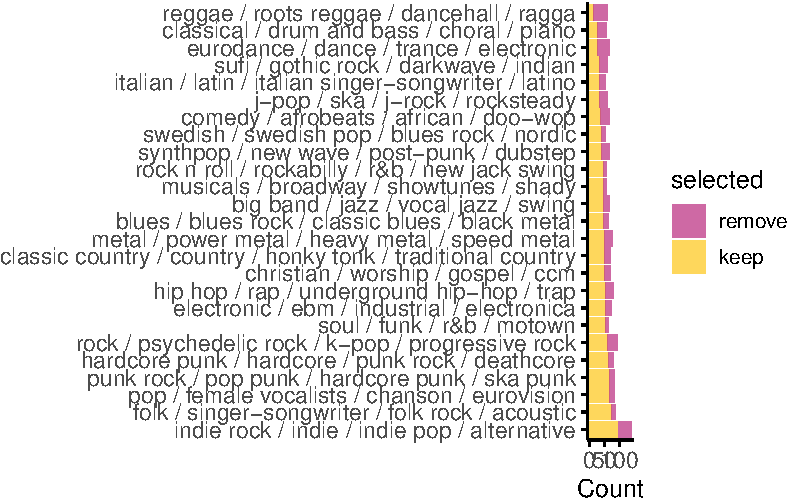
\includegraphics[keepaspectratio]{manuscript_files/figure-pdf/screening_by_genre-1.pdf}}

{Note. ``Remove'' indicates songs excluded due to screening criteria.}

\begin{Shaded}
\begin{Highlighting}[]
\FunctionTok{make\_apa\_freq\_table}\NormalTok{(}
\NormalTok{  lyrics\_df}\SpecialCharTok{|\textgreater{}}\FunctionTok{rename}\NormalTok{(}\StringTok{\textasciigrave{}}\AttributeTok{Artist Topic Tags}\StringTok{\textasciigrave{}}\OtherTok{=}\NormalTok{artist\_topic\_bin\_labels),}
  \StringTok{\textasciigrave{}}\AttributeTok{Artist Topic Tags}\StringTok{\textasciigrave{}}\NormalTok{,}
  \AttributeTok{title =} \FunctionTok{md}\NormalTok{(}\StringTok{"**Table s{-}5**"}\NormalTok{),}
  \AttributeTok{subtitle =} \FunctionTok{md}\NormalTok{(}\StringTok{"*Frequencies by artist topic*"}\NormalTok{)}
\NormalTok{)}
\end{Highlighting}
\end{Shaded}

\begin{table}
\caption*{
{\large \textbf{Table s-5}} \\ 
{\small \emph{Frequencies by artist topic}}
} 
\fontsize{9.0pt}{10.8pt}\selectfont
\begin{tabular*}{\linewidth}{@{\extracolsep{\fill}}lrrr}
\toprule
{Artist Topic Tags} & Removed & Kept & Total n \\ 
\midrule\addlinespace[2.5pt]
reggae / roots reggae / dancehall / ragga & 49 (79.0\%) & 13 (21.0\%) & 62 \\ 
indie rock / indie / indie pop / alternative & 44 (31.4\%) & 96 (68.6\%) & 140 \\ 
eurodance / dance / trance / electronic & 40 (58.8\%) & 28 (41.2\%) & 68 \\ 
rock / psychedelic rock / k-pop / progressive rock & 31 (33.3\%) & 62 (66.7\%) & 93 \\ 
classical / drum and bass / choral / piano & 30 (52.6\%) & 27 (47.4\%) & 57 \\ 
comedy / afrobeats / african / doo-wop & 28 (42.4\%) & 38 (57.6\%) & 66 \\ 
sufi / gothic rock / darkwave / indian & 27 (45.0\%) & 33 (55.0\%) & 60 \\ 
synthpop / new wave / post-punk / dubstep & 27 (40.3\%) & 40 (59.7\%) & 67 \\ 
hip hop / rap / underground hip-hop / trap & 26 (32.5\%) & 54 (67.5\%) & 80 \\ 
j-pop / ska / j-rock / rocksteady & 26 (43.3\%) & 34 (56.7\%) & 60 \\ 
metal / power metal / heavy metal / speed metal & 25 (32.9\%) & 51 (67.1\%) & 76 \\ 
electronic / ebm / industrial / electronica & 21 (28.0\%) & 54 (72.0\%) & 75 \\ 
italian / latin / italian singer-songwriter / latino & 21 (38.9\%) & 33 (61.1\%) & 54 \\ 
big band / jazz / vocal jazz / swing & 20 (29.9\%) & 47 (70.1\%) & 67 \\ 
classic country / country / honky tonk / traditional country & 19 (27.1\%) & 51 (72.9\%) & 70 \\ 
christian / worship / gospel / ccm & 18 (25.7\%) & 52 (74.3\%) & 70 \\ 
hardcore punk / hardcore / punk rock / deathcore & 16 (20.0\%) & 64 (80.0\%) & 80 \\ 
pop / female vocalists / chanson / eurovision & 16 (19.0\%) & 68 (81.0\%) & 84 \\ 
punk rock / pop punk / hardcore punk / ska punk & 16 (19.3\%) & 67 (80.7\%) & 83 \\ 
swedish / swedish pop / blues rock / nordic & 16 (29.1\%) & 39 (70.9\%) & 55 \\ 
blues / blues rock / classic blues / black metal & 15 (23.8\%) & 48 (76.2\%) & 63 \\ 
folk / singer-songwriter / folk rock / acoustic & 15 (16.9\%) & 74 (83.1\%) & 89 \\ 
rock n roll / rockabilly / r\&b / new jack swing & 12 (20.7\%) & 46 (79.3\%) & 58 \\ 
musicals / broadway / showtunes / shady & 11 (19.3\%) & 46 (80.7\%) & 57 \\ 
soul / funk / r\&b / motown & 10 (15.4\%) & 55 (84.6\%) & 65 \\ 
\bottomrule
\end{tabular*}
\end{table}

\paragraph{Topic}\label{topic}

Topic modelling resulted in imprecise lyrical topics, which
\textcite{demetriou2024towards} included as a further means to diversify
the sample of lyrics. Although no precise definition of each topic could
be derived, the team agreed on the following approximations of \(8\)
included lyric topics. Songs overwhelmingly fell categories relating to
sadness and romance, a topic the original team felt was split into two
groupings \texttt{sad/romantic1} and \texttt{sad/romantic2}.

{\textbf{Figure s-4}\\
\emph{Manual screening outcome by lyric topic}}

\begin{Shaded}
\begin{Highlighting}[]
\FunctionTok{make\_removed\_counts}\NormalTok{(lyrics\_df, topic\_label)}
\end{Highlighting}
\end{Shaded}

\pandocbounded{
\includegraphics[keepaspectratio]{manuscript_files/figure-pdf/unnamed-chunk-48-1.pdf}}

\subsubsection{Skew Correction}\label{skew-correction}

\textcite{demetriou2024towards} observed a skew in data concentration
such that songs that were recent and artists that appeared very
frequently in playlists were most likely be sampled. To compensate,
\textcite{demetriou2024towards} oversampled less populated bins by
increasing the probability that songs in underpopulated bins are
selected, using a maximum-a-posteriori (MAP) estimate of the categorical
distribution of each stratum \autocite{bassett2019maximum}. Oversampling
is controlled via a concentration parameter \(a\) of the symmetric
Dirichlet distribution which was heuristically set to 40,000, with the
aim of between 5\% and 10\% of the overall pool of 2200 songs being
drawn from underpopulated bins.

\subsubsection{Mislabelled `Kept' Songs}\label{mislabelled-kept-songs}

We observe 19 songs in the 380 songs used by
\textcite{demetriou2024towards}, whereby 19 songs are labelled
``remove'' but also ``wave\_1'', which suggests that those 19 songs were
either included erroneously, or mislabeled ``remove'' erroneously. We
elected not to use those 19 songs.

\subsection{Political Speech Stimuli}\label{political-speech-stimuli}

We sampled U.S. State of the Union addresses (post-1900) from the UVA
Miller Center archive. Speeches were sampled across two strata: (1)
President and (2) speech, both of which were labelled by the Miller
center. Speeches were stratified by president and by individual address
so that each president contributed a comparable number of excerpts.
Presidents with fewer addresses contributed more chunks per speech,
while those with many addresses contributed fewer. Each chunk yielded
the first \textasciitilde200 words (ending at a sentence boundary),
producing an approximately balanced set of excerpts across presidents
and speeches. The final pool comprised 300 excerpts for the main study
and 13 each for two pilot studies. Details of the average number of
excerpts by party for both the initial pool and sample are shown in
Table 5. Visualization of number of speeches per president are shown in
Figure 5.

Repository of sampling procedure can be found here:
https://github.com/Gargant0373/PresidentialSpeechSampling/blob/master/sample.py

{\textbf{Figure s-5}\\
\emph{Number of speech excerpts per President}}

\begin{Shaded}
\begin{Highlighting}[]
\NormalTok{colors }\OtherTok{\textless{}{-}} \FunctionTok{viridis}\NormalTok{(}\DecValTok{10}\NormalTok{) }

\NormalTok{speech\_df }\SpecialCharTok{|\textgreater{}} 
  
  \FunctionTok{filter}\NormalTok{(id }\SpecialCharTok{\%in\%}\NormalTok{ speech\_IDs) }\SpecialCharTok{|\textgreater{}}
  
  \FunctionTok{count}\NormalTok{(president, party, }\AttributeTok{name =} \StringTok{"n"}\NormalTok{) }\SpecialCharTok{|\textgreater{}}
  
  \FunctionTok{mutate}\NormalTok{(}\AttributeTok{president =} \FunctionTok{fct\_reorder}\NormalTok{(president, n, }\AttributeTok{.desc =}\NormalTok{ T)) }\SpecialCharTok{|\textgreater{}}
  
  \FunctionTok{ggplot}\NormalTok{(}\FunctionTok{aes}\NormalTok{(}\AttributeTok{x =}\NormalTok{ president, }\AttributeTok{y =}\NormalTok{ n, }\AttributeTok{fill =}\NormalTok{ party)) }\SpecialCharTok{+}
    \FunctionTok{geom\_col}\NormalTok{(}\AttributeTok{alpha =}\NormalTok{ .}\DecValTok{75}\NormalTok{) }\SpecialCharTok{+}
    \FunctionTok{coord\_flip}\NormalTok{() }\SpecialCharTok{+}
    \FunctionTok{labs}\NormalTok{(}\AttributeTok{x =} \ConstantTok{NULL}\NormalTok{, }\AttributeTok{y =} \StringTok{"Count"}\NormalTok{) }\SpecialCharTok{+}
    \FunctionTok{scale\_fill\_manual}\NormalTok{(}\AttributeTok{values =} \FunctionTok{c}\NormalTok{(colors[}\DecValTok{5}\NormalTok{], colors[}\DecValTok{9}\NormalTok{])) }\SpecialCharTok{+} 
    \FunctionTok{theme\_apa}\NormalTok{()}
\end{Highlighting}
\end{Shaded}

\pandocbounded{
\includegraphics[keepaspectratio]{manuscript_files/figure-pdf/unnamed-chunk-49-1.pdf}}

\begin{Shaded}
\begin{Highlighting}[]
\NormalTok{df }\OtherTok{\textless{}{-}}\NormalTok{ speech\_df}

\CommentTok{\# function to summarize by party}
\NormalTok{summarise\_party }\OtherTok{\textless{}{-}} \ControlFlowTok{function}\NormalTok{(data) \{}
\NormalTok{  data }\SpecialCharTok{\%\textgreater{}\%}
    \FunctionTok{group\_by}\NormalTok{(party) }\SpecialCharTok{\%\textgreater{}\%}
    \FunctionTok{summarise}\NormalTok{(}
      \AttributeTok{n\_excerpts    =} \FunctionTok{n}\NormalTok{(),}
      \AttributeTok{n\_speeches    =} \FunctionTok{n\_distinct}\NormalTok{(url),}
      \AttributeTok{n\_presidents  =} \FunctionTok{n\_distinct}\NormalTok{(president),}
      \AttributeTok{.groups =} \StringTok{"drop"}
\NormalTok{    ) }\SpecialCharTok{\%\textgreater{}\%}
    \FunctionTok{mutate}\NormalTok{(}
      \AttributeTok{excerpts\_per\_president =}\NormalTok{ n\_excerpts }\SpecialCharTok{/}\NormalTok{ n\_presidents,}
      \AttributeTok{pct\_excerpts =}\NormalTok{ n\_excerpts }\SpecialCharTok{/} \FunctionTok{sum}\NormalTok{(n\_excerpts))\}}

\CommentTok{\# 1) Full pool}
\NormalTok{full\_summary }\OtherTok{\textless{}{-}} \FunctionTok{summarise\_party}\NormalTok{(df) }\SpecialCharTok{\%\textgreater{}\%}
  \FunctionTok{mutate}\NormalTok{(}\AttributeTok{sample =} \StringTok{"Initial pool"}\NormalTok{)}

\CommentTok{\# 2) Annotated subsample}
\NormalTok{sub\_df }\OtherTok{\textless{}{-}}\NormalTok{ df }\SpecialCharTok{\%\textgreater{}\%} \FunctionTok{filter}\NormalTok{(id }\SpecialCharTok{\%in\%}\NormalTok{ speech\_IDs)}
\NormalTok{sub\_summary }\OtherTok{\textless{}{-}} \FunctionTok{summarise\_party}\NormalTok{(sub\_df) }\SpecialCharTok{\%\textgreater{}\%}
  \FunctionTok{mutate}\NormalTok{(}\AttributeTok{sample =} \StringTok{"Sample"}\NormalTok{)}

\CommentTok{\# 3) Combine}
\NormalTok{combined\_summary }\OtherTok{\textless{}{-}} \FunctionTok{bind\_rows}\NormalTok{(full\_summary, sub\_summary) }\SpecialCharTok{\%\textgreater{}\%}
  \FunctionTok{relocate}\NormalTok{(sample, }\AttributeTok{.before =}\NormalTok{ party)}

\CommentTok{\# 4) Render as gt table}
\NormalTok{combined\_summary }\SpecialCharTok{\%\textgreater{}\%}
  \FunctionTok{gt}\NormalTok{(}\AttributeTok{groupname\_col =} \StringTok{"sample"}\NormalTok{) }\SpecialCharTok{\%\textgreater{}\%}   
    \FunctionTok{tab\_header}\NormalTok{(}
    \AttributeTok{title =} \FunctionTok{md}\NormalTok{(}\StringTok{"**Table s{-}6**"}\NormalTok{),   }
    \AttributeTok{subtitle =} \FunctionTok{md}\NormalTok{(}\StringTok{"*Descriptive statistics of speech excerpts by party*"}\NormalTok{)) }\SpecialCharTok{|\textgreater{}}
  \FunctionTok{cols\_label}\NormalTok{(}
    \AttributeTok{party =} \StringTok{"Party"}\NormalTok{,}
    \AttributeTok{n\_excerpts =} \StringTok{"Total excerpts"}\NormalTok{,}
    \AttributeTok{n\_speeches =} \StringTok{"Unique speeches"}\NormalTok{,}
    \AttributeTok{n\_presidents =} \StringTok{"Unique presidents"}\NormalTok{,}
    \AttributeTok{excerpts\_per\_president =} \StringTok{"Avg. excerpts per president"}\NormalTok{,}
    \AttributeTok{pct\_excerpts =} \StringTok{"\% of all excerpts"}\NormalTok{) }\SpecialCharTok{\%\textgreater{}\%}
  
  \FunctionTok{fmt\_number}\NormalTok{(}\AttributeTok{columns =} \FunctionTok{c}\NormalTok{(n\_excerpts, n\_speeches, n\_presidents), }\AttributeTok{decimals =} \DecValTok{0}\NormalTok{) }\SpecialCharTok{\%\textgreater{}\%}
  \FunctionTok{fmt\_number}\NormalTok{(}\AttributeTok{columns =}\NormalTok{ excerpts\_per\_president, }\AttributeTok{decimals =} \DecValTok{1}\NormalTok{) }\SpecialCharTok{\%\textgreater{}\%}
  \FunctionTok{fmt\_percent}\NormalTok{(}\AttributeTok{columns =}\NormalTok{ pct\_excerpts, }\AttributeTok{decimals =} \DecValTok{1}\NormalTok{) }\SpecialCharTok{\%\textgreater{}\%}
  
  \FunctionTok{tab\_options}\NormalTok{(}
    \AttributeTok{table.font.size =} \DecValTok{12}\NormalTok{,}
    \AttributeTok{heading.align =} \StringTok{"left"}\NormalTok{,    }
    \AttributeTok{table\_body.hlines.width =} \FunctionTok{px}\NormalTok{(}\DecValTok{0}\NormalTok{),}
    \AttributeTok{table.border.top.width =} \FunctionTok{px}\NormalTok{(}\DecValTok{0}\NormalTok{),}
    \AttributeTok{table.border.bottom.width =} \FunctionTok{px}\NormalTok{(}\DecValTok{1}\NormalTok{),}
    \AttributeTok{column\_labels.border.top.width =} \FunctionTok{px}\NormalTok{(}\DecValTok{0}\NormalTok{),}
    \AttributeTok{column\_labels.border.bottom.width =} \FunctionTok{px}\NormalTok{(}\DecValTok{1}\NormalTok{)) }\SpecialCharTok{\%\textgreater{}\%}
  
  \FunctionTok{tab\_style}\NormalTok{(}
    \AttributeTok{style =} \FunctionTok{cell\_text}\NormalTok{(}\AttributeTok{align =} \StringTok{"center"}\NormalTok{, }\AttributeTok{whitespace =} \StringTok{"pre{-}wrap"}\NormalTok{),}
    \AttributeTok{locations =} \FunctionTok{cells\_column\_labels}\NormalTok{(}\FunctionTok{everything}\NormalTok{())) }\SpecialCharTok{|\textgreater{}}
  
  \FunctionTok{cols\_width}\NormalTok{(}
\NormalTok{    party }\SpecialCharTok{\textasciitilde{}} \FunctionTok{px}\NormalTok{(}\DecValTok{100}\NormalTok{),}
\NormalTok{    n\_excerpts }\SpecialCharTok{\textasciitilde{}} \FunctionTok{px}\NormalTok{(}\DecValTok{100}\NormalTok{),}
\NormalTok{    n\_speeches }\SpecialCharTok{\textasciitilde{}} \FunctionTok{px}\NormalTok{(}\DecValTok{100}\NormalTok{),}
\NormalTok{    n\_presidents }\SpecialCharTok{\textasciitilde{}}\NormalTok{ (}\DecValTok{100}\NormalTok{), }
\NormalTok{    excerpts\_per\_president }\SpecialCharTok{\textasciitilde{}} \FunctionTok{px}\NormalTok{(}\DecValTok{100}\NormalTok{),}
\NormalTok{    pct\_excerpts }\SpecialCharTok{\textasciitilde{}} \FunctionTok{px}\NormalTok{(}\DecValTok{100}\NormalTok{)) }\SpecialCharTok{\%\textgreater{}\%}
    
  \FunctionTok{tab\_style}\NormalTok{(}
    \AttributeTok{style =} \FunctionTok{cell\_text}\NormalTok{(}\AttributeTok{align =} \StringTok{"center"}\NormalTok{),}
    \AttributeTok{locations =} \FunctionTok{cells\_row\_groups}\NormalTok{()) }\SpecialCharTok{\%\textgreater{}\%}
  
  \FunctionTok{cols\_align}\NormalTok{(}\AttributeTok{align =} \StringTok{"center"}\NormalTok{, }\AttributeTok{columns =} \FunctionTok{everything}\NormalTok{())}
\end{Highlighting}
\end{Shaded}

\begin{table}
\caption*{
{\large \textbf{Table s-6}} \\ 
{\small \emph{Descriptive statistics of speech excerpts by party}}
} 
\fontsize{9.0pt}{10.8pt}\selectfont
\begin{tabular*}{\linewidth}{@{\extracolsep{\fill}}>{\centering\arraybackslash}p{\dimexpr 75.00pt -2\tabcolsep-1.5\arrayrulewidth}>{\centering\arraybackslash}p{\dimexpr 75.00pt -2\tabcolsep-1.5\arrayrulewidth}>{\centering\arraybackslash}p{\dimexpr 75.00pt -2\tabcolsep-1.5\arrayrulewidth}>{\centering\arraybackslash}p{\dimexpr 75.00pt -2\tabcolsep-1.5\arrayrulewidth}>{\centering\arraybackslash}p{\dimexpr 75.00pt -2\tabcolsep-1.5\arrayrulewidth}>{\centering\arraybackslash}p{\dimexpr 75.00pt -2\tabcolsep-1.5\arrayrulewidth}}
\toprule
Party & Total excerpts & Unique speeches & Unique presidents & Avg. excerpts per president & \% of all excerpts \\ 
\midrule\addlinespace[2.5pt]
\multicolumn{6}{l}{{Initial pool}} \\[2.5pt] 
\midrule\addlinespace[2.5pt]
Democratic & 499 & 63 & 9 & 55.4 & 43.0\% \\ 
Republican & 662 & 66 & 12 & 55.2 & 57.0\% \\ 
\midrule\addlinespace[2.5pt]
\multicolumn{6}{l}{{Sample}} \\[2.5pt] 
\midrule\addlinespace[2.5pt]
Democratic & 146 & 58 & 9 & 16.2 & 44.8\% \\ 
Republican & 180 & 64 & 12 & 15.0 & 55.2\% \\ 
\bottomrule
\end{tabular*}
\end{table}

\subsection{Word Counts}\label{word-counts}

\begin{Shaded}
\begin{Highlighting}[]
\NormalTok{lyrics\_summary }\OtherTok{\textless{}{-}}\NormalTok{ lyrics\_df }\SpecialCharTok{|\textgreater{}} \FunctionTok{filter}\NormalTok{(item\_ID }\SpecialCharTok{\%in\%}\NormalTok{ lyrics\_IDs) }\SpecialCharTok{|\textgreater{}} 
  \FunctionTok{summarize}\NormalTok{(}\AttributeTok{mean =} \FunctionTok{mean}\NormalTok{(word\_count), }\AttributeTok{sd =} \FunctionTok{sd}\NormalTok{(word\_count))}

\NormalTok{speech\_summary }\OtherTok{\textless{}{-}}\NormalTok{ speech\_df }\SpecialCharTok{|\textgreater{}} \FunctionTok{filter}\NormalTok{(id }\SpecialCharTok{\%in\%}\NormalTok{ speech\_IDs) }\SpecialCharTok{|\textgreater{}} 
  \FunctionTok{summarize}\NormalTok{(}\AttributeTok{mean =} \FunctionTok{mean}\NormalTok{(word\_count), }\AttributeTok{sd =} \FunctionTok{sd}\NormalTok{(word\_count))}
\end{Highlighting}
\end{Shaded}

Distributions of word counts differ substantially between song lyrics
and speeches. All lyrics were truncated to the first 30\% as estimated
by Musixmatch, the word counts vary substantially more than the speech
excerpts, where our process for determining an excerpt truncated to the
nearest complete sentence after 200 words. On average, speech excerpts
were longer (\emph{M} = 246.6, \emph{SD} = 12.5 words) than lyric
excerpts (\emph{M} = 82.8, \emph{SD} = 45.4 words).

{\textbf{Figure 6}\\
\emph{Density plot of word counts in speech and lyric excerpts}}

\begin{Shaded}
\begin{Highlighting}[]
\NormalTok{df }\OtherTok{\textless{}{-}} \FunctionTok{bind\_rows}\NormalTok{(}
\NormalTok{  lyrics\_df }\SpecialCharTok{|\textgreater{}} \FunctionTok{filter}\NormalTok{(item\_ID }\SpecialCharTok{\%in\%}\NormalTok{ lyrics\_IDs) }\SpecialCharTok{|\textgreater{}} 
    \FunctionTok{select}\NormalTok{(item\_ID, word\_count) }\SpecialCharTok{|\textgreater{}} \FunctionTok{mutate}\NormalTok{(}\AttributeTok{source =} \StringTok{"Lyrics"}\NormalTok{, }\AttributeTok{item\_ID =} \FunctionTok{as.character}\NormalTok{(item\_ID)), }
\NormalTok{  speech\_df }\SpecialCharTok{|\textgreater{}} \FunctionTok{filter}\NormalTok{(id }\SpecialCharTok{\%in\%}\NormalTok{ speech\_IDs) }\SpecialCharTok{|\textgreater{}} 
    \FunctionTok{select}\NormalTok{(id, word\_count) }\SpecialCharTok{|\textgreater{}} \FunctionTok{rename}\NormalTok{(}\AttributeTok{item\_ID =}\NormalTok{ id) }\SpecialCharTok{|\textgreater{}}
    \FunctionTok{mutate}\NormalTok{(}\AttributeTok{source =} \StringTok{"Speeches"}\NormalTok{)) }

\NormalTok{df }\SpecialCharTok{|\textgreater{}}
  
  \FunctionTok{ggplot}\NormalTok{(}\FunctionTok{aes}\NormalTok{(}\AttributeTok{x =}\NormalTok{ word\_count, }\AttributeTok{fill =}\NormalTok{ source)) }\SpecialCharTok{+}
    \FunctionTok{geom\_density}\NormalTok{(}\AttributeTok{alpha =} \FloatTok{0.7}\NormalTok{) }\SpecialCharTok{+}
  \FunctionTok{scale\_fill\_manual}\NormalTok{(}\AttributeTok{values =} \FunctionTok{c}\NormalTok{(}\StringTok{"Speeches"} \OtherTok{=} \StringTok{"\#21908C"}\NormalTok{, }\StringTok{"Lyrics"} \OtherTok{=} \StringTok{"\#440154"}\NormalTok{)) }\SpecialCharTok{+}
    \FunctionTok{labs}\NormalTok{(}
    \AttributeTok{x =} \StringTok{"Word count"}\NormalTok{,}
    \AttributeTok{y =} \StringTok{"Density"}\NormalTok{) }\SpecialCharTok{+}
  \FunctionTok{theme\_apa}\NormalTok{()}
\end{Highlighting}
\end{Shaded}

\pandocbounded{
\includegraphics[keepaspectratio]{manuscript_files/figure-pdf/unnamed-chunk-52-1.pdf}}

\section{Appendix B: Survey}\label{appendix-b-survey}

\subsection{SSVS Instructions for
participants}\label{ssvs-instructions-for-participants}

``In this questionnaire you are to ask yourself:

``What values are important to ME as guiding principles in MY life, and
what values are less important to me?''

There is a list of values on the following page. These values come from
different cultures. In the parentheses following each value is an
explanation that may help you to understand its meaning. Your task is to
rate how important each value is for you as a guiding principle in your
life.

Use the rating scale below:

0 means the value is not at all important, it is not relevant as a
guiding principle for you. 3 means the value is important. 6 means the
value is very important.

The higher the number (0, 1, 2, 3, 4, 5, 6, 7), the more important the
value is as a guiding principle in YOUR life.

-1 is for rating any values opposed to the principles that guide you. 7
is for rating a value of supreme importance as a guiding principle in
your life; Ordinarily there are no more than two such values.

On the scale next to each value, indicate the number
(-1,0,1,2,3,4,5,6,7) that indicates the importance of that value for
you, personally. Try to distinguish as much as possible between the
values by using all the numbers.

You may need to use numbers more than once.''

\subsection{Task Instructions}\label{task-instructions}

\subsubsection{Lyrics}\label{lyrics}

\paragraph{General Instructions:}\label{general-instructions}

``In the main part of this survey, you will be shown parts of song
lyrics from 15 songs, and asked to complete similar questions about the
values you perceive them.

IMPORTANT: Lyrics can be written from different perspectives, some of
which are not the same as the writer of the lyrics. In other words, the
AUTHOR of the lyrics may choose a SPEAKER for their lyrics that is not
themselves.

The SPEAKER of the lyrics could be a fictional character, a real person
from history or the present other than the author, or even an imaginary
object. And of course it could be the AUTHOR themselves. Please read the
lyrics, and answer the questions while thinking about the SPEAKER.

Do not look up the lyrics elsewhere.

Ask yourself: ``What values are important to the SPEAKER as guiding
principles in in their life, and what values are less important to them?
Use the same rating scale that you used in the questionnaire earlier: 0
means the value is not at all important. 3 means the value is important.
6 means the value is very important. -1 means the value is opposed to
the principles that guide the SPEAKER. 7 means the value is of supreme
importance as the guiding principle in the SPEAKER's life.

Please start by rating the value you feel is the most important to the
SPEAKER with a 6 or 7, and the value that is most opposed to their
values with a -1 or 0, (green arrows).Then complete the scales for the
remainder of the values. Indicate NA (red arrow) if you feel the SPEAKER
doesn't describe how they feel about that value. Try to distinguish as
much as possible between the values by using all the numbers. You may
need to use numbers more than once, but try not to.''

\paragraph{Post-Quiz Final
Instructions:}\label{post-quiz-final-instructions}

``Thanks! We'll now ask you to respond to our questions about 15 song
lyrics. Please read only the lyrics between the quotes, do not search
them on the internet or look them up elsewhere. Think about the SPEAKER
of the lyrics, and answer the questions with them in mind.

Please click on the arrow below when you are ready.

WARNING: These lyrics are randomly selected from popular music, some of
which use offensive language or describe offensive situations.''

\paragraph{Question Instructions:}\label{question-instructions}

``Between the quotation marks below are some song lyrics. Please take a
moment to read them and think about the SPEAKER the lyrics. Please
remember that this SPEAKER might be a the AUTHOR themselves, or someone
or something else:''

\paragraph{Attention Test}\label{attention-test}

``This song lyric is actually a test to see if you are paying attention
Please indicate that the Speaker and Author are the same person, That
you are not familiar with this song, indicate that this Speaker values
STIMULATION at 7, and please set all other values to 0''

\subsubsection{Speeches}\label{speeches}

\paragraph{General Instructions:}\label{general-instructions-1}

``You will now be shown 15 pieces of U.S. Presidential Speeches, and
asked to complete similar questions about the values you perceive in
them.

IMPORTANT: Some speeches were delivered in written form, and some were
delivered as speeches. Sometimes, the transcript refers to dialogue from
people other than the U.S. President, laughter, or contains other
indications. In our questions, we refer to the SPEAKER, which is always
the U.S. President delivering the speech.

Please read the piece of the speech, and answer the questions while
thinking about the SPEAKER and their words.

Please do not look up the speeches elsewhere.

Ask yourself: ``What values are important to the SPEAKER as guiding
principles in in their life, and what values are less important to them?
Use the same rating scale that you used in the questionnaire earlier: 0
means the value is not at all important. 3 means the value is important.
6 means the value is very important. -1 means the value is opposed to
the principles that guide the SPEAKER. 7 means the value is of supreme
importance as the guiding principle in the SPEAKER's life.

Please start by rating the value you feel is the most important to the
SPEAKER with a 6 or 7, and the value that is most opposed to their
values with a -1 or 0, (green arrows). Then complete the scales for the
remainder of the values. Indicate NA (red arrow) if you feel the SPEAKER
doesn't describe how they feel about that value.

Try to distinguish as much as possible between the values by using all
the numbers. You may need to use numbers more than once.''

\paragraph{Post-Quiz Final
Instructions:}\label{post-quiz-final-instructions-1}

``Thanks! We'll now ask you to respond to our questions about 15 parts
from U.S. Presidential speeches. Please read only the parts of the
speeches between the quotes, do not search them on the internet or look
them up elsewhere. Think about the SPEAKER of the speech, the U.S.
president, and answer the questions with them in mind.

Please click on the arrow below when you are ready.

WARNING: These speeches were randomly selected, some of which use
language that might have been acceptable at the time, but would be
considered offensive today.''

\paragraph{Question Instructions:}\label{question-instructions-1}

``Between the quotation marks below are parts of a U.S. Presidential
Speech. Please take a moment to read them and think about the SPEAKER of
the speech.''

\paragraph{Attention Test:}\label{attention-test-1}

``This speech part is actually a test to see if you are paying
attention. Please indicate that you are not familiar with this
president, that the president is a Republican. Indicate that this
Speaker values STIMULATION at 7, and please set all other values to 0.''

\subsection{Debrief}\label{debrief}

\subsubsection{Lyrics}\label{lyrics-1}

``Thanks for completing the survey!

Our research group, and other scientists like us, are interested in
perceived personal values in song lyrics.

By `values', we mean the abstract concepts or beliefs that we feel are
important as life-guide principles. They have been shown to be related
to our behaviors and goals at the most abstract level, above and beyond
any specific situation. According to Shalom Schwartz, there are 10 main
values that all people share, and each person has their own ranking of
these values. In more recent work, these are broken up further into 19
values, but we used a shorter 10-item version.

This study is helping us learn how to gather data from people about the
values that they think song lyrics express. Our questionnaire about
values is based on one that was a part of the European Social Survey,
and later shortened. You responded to it about yourself at the start of
the study. Respondents like yourself then also completed it about what
they thought of the values of the `speaker' of each song lyric. We will
analyze the data to see whether our version of this questionnaire is
also useful for gathering information on song lyrics.

We expect that different people will interpret the values of lyrics
differently. People might have a preference for different genres of
music or prioritize different values in their lives. People with
different backgrounds (e.g.~ethnicity, gender, level of education, age)
or who prioritize different values might also interpret song lyrics
differently. We used various options on the Prolific platform to screen
respondents like yourself, and also asked a number of questions, to
explore whether any of these factors make a difference in the way people
interpret the values of song lyrics.

Knowing our reasons for the study might have changed the way you would
answer the questions in this survey. For this reason, we only explain
the reasons for our study at the end.

Some songs have lyrics that are difficult or impossible to interpret. We
asked about your confidence in your ratings, to see if some songs are
more vague, or ambiguous than others. We also asked about how subjective
you thought the task was overall, to help us estimate how many
participants we might need for future studies.

De-identified data from this study may be part of published academic
work in the future. We will not include personally identifying
information (e.g.~your Prolific ID), but it will include your responses
to questions about the song lyrics, your music preferences,
demographics, and values. We'd like to remind you that you can request
to withdraw your data at any time by emailing a.m.demetriou@tudelft.nl.
Please be aware that as time passess this will become more challenging
especially if work from this study has been published. We will make all
necessary efforts to remove it, but there is always a risk that we will
not recover every instance of it after it has been published.

Thanks again for participating! Please let us know if you have any
feedback for us below. NOTE: Please do not enter any identifying or
sensitive information in the field.''

\subsubsection{Speeches}\label{speeches-1}

``Thanks for completing the survey!

Our research group, and other scientists like us, are interested in
perceived personal values in text, like political speeches. By `values',
we mean the abstract concepts or beliefs that we feel are important as
life-guide principles. They have been shown to be related to our
behaviors and goals at the most abstract level, above and beyond any
specific situation. According to Shalom Schwartz, there are 10 main
values that all people share, and each person has their own ranking of
these values. In more recent work, these are broken up further into 19
values, but we used a shorter 10-item version.

This study is helping us learn how to gather data from people about the
values that they think political speeches express. Our questionnaire
about values is based on one that was a part of the European Social
Survey, and later shortened. Respondents like yourself completed it
about what they thought of the values of the `speaker' in song lyrics in
a prior study. In this study, we will analyze the data to see whether
our version of this questionnaire is also useful for gathering
information on political speeches. We expect that different people will
interpret the values of speeches differently. People with different
backgrounds (e.g.~ethnicity, gender, level of education, age), or
political affiliations might also interpret speeches differently. We used
various options on the Prolific platform to screen respondents like
yourself, to explore whether any of these factors make a difference in
the way people interpret the values in speeches.

Knowing our reasons for the study might have changed the way you would
answer the questions in this survey. For this reason, we only explain
the reasons for our study at the end. Some parts of speeches taken out
of context are difficult or impossible to interpret. We asked about your
confidence in your ratings, to see if some excerpts are more vague, or
ambiguous than others. We also asked about how subjective you thought
the task was overall, to help us estimate how many participants we might
need for future studies.

De-identified data from this study may be part of published academic
work in the future. We will not include personally identifying
information (e.g.~your Prolific ID), but it will include your responses
to questions about the song lyrics, your music preferences,
demographics, and values. We'd like to remind you that you can request
to withdraw your data at any time by emailing a.m.demetriou@tudelft.nl.
Please be aware that as time passess this will become more challenging
especially if work from this study has been published. We will make all
necessary efforts to remove it, but there is always a risk that we will
not recover every instance of it after it has been published.

Thanks again for participating! Please let us know if you have any
feedback for us below. Please do not enter any identifying or sensitive
information in the field.''





\end{document}
